\documentclass[]{article}
\usepackage{lmodern}
\usepackage{amssymb,amsmath}
\usepackage{ifxetex,ifluatex}
\usepackage{fixltx2e} % provides \textsubscript
\ifnum 0\ifxetex 1\fi\ifluatex 1\fi=0 % if pdftex
  \usepackage[T1]{fontenc}
  \usepackage[utf8]{inputenc}
\else % if luatex or xelatex
  \ifxetex
    \usepackage{mathspec}
  \else
    \usepackage{fontspec}
  \fi
  \defaultfontfeatures{Ligatures=TeX,Scale=MatchLowercase}
\fi
% use upquote if available, for straight quotes in verbatim environments
\IfFileExists{upquote.sty}{\usepackage{upquote}}{}
% use microtype if available
\IfFileExists{microtype.sty}{%
\usepackage{microtype}
\UseMicrotypeSet[protrusion]{basicmath} % disable protrusion for tt fonts
}{}
\usepackage[margin=1in]{geometry}
\usepackage{hyperref}
\hypersetup{unicode=true,
            pdftitle={Good Empirics Dominate Bad Theory: Comments on Blair and Sambanis, 2020, ``Forecasting Civil Wars: Theory and Structure in an Age of `Big Data' and Machine Learning'', JCR},
            pdfauthor={Richard K. Morgan and Andreas Beger and Michael D. Ward},
            pdfborder={0 0 0},
            breaklinks=true}
\urlstyle{same}  % don't use monospace font for urls
\usepackage{longtable,booktabs}
\usepackage{graphicx,grffile}
\makeatletter
\def\maxwidth{\ifdim\Gin@nat@width>\linewidth\linewidth\else\Gin@nat@width\fi}
\def\maxheight{\ifdim\Gin@nat@height>\textheight\textheight\else\Gin@nat@height\fi}
\makeatother
% Scale images if necessary, so that they will not overflow the page
% margins by default, and it is still possible to overwrite the defaults
% using explicit options in \includegraphics[width, height, ...]{}
\setkeys{Gin}{width=\maxwidth,height=\maxheight,keepaspectratio}
\IfFileExists{parskip.sty}{%
\usepackage{parskip}
}{% else
\setlength{\parindent}{0pt}
\setlength{\parskip}{6pt plus 2pt minus 1pt}
}
\setlength{\emergencystretch}{3em}  % prevent overfull lines
\providecommand{\tightlist}{%
  \setlength{\itemsep}{0pt}\setlength{\parskip}{0pt}}
\setcounter{secnumdepth}{0}
% Redefines (sub)paragraphs to behave more like sections
\ifx\paragraph\undefined\else
\let\oldparagraph\paragraph
\renewcommand{\paragraph}[1]{\oldparagraph{#1}\mbox{}}
\fi
\ifx\subparagraph\undefined\else
\let\oldsubparagraph\subparagraph
\renewcommand{\subparagraph}[1]{\oldsubparagraph{#1}\mbox{}}
\fi

%%% Use protect on footnotes to avoid problems with footnotes in titles
\let\rmarkdownfootnote\footnote%
\def\footnote{\protect\rmarkdownfootnote}

%%% Change title format to be more compact
\usepackage{titling}

% Create subtitle command for use in maketitle
\providecommand{\subtitle}[1]{
  \posttitle{
    \begin{center}\large#1\end{center}
    }
}

\setlength{\droptitle}{-2em}

  \title{Good Empirics Dominate Bad Theory: Comments on Blair and Sambanis, 2020,
``Forecasting Civil Wars: Theory and Structure in an Age of `Big Data'
and Machine Learning'', \emph{JCR}}
    \pretitle{\vspace{\droptitle}\centering\huge}
  \posttitle{\par}
    \author{Richard K. Morgan and Andreas Beger and Michael D. Ward}
    \preauthor{\centering\large\emph}
  \postauthor{\par}
      \predate{\centering\large\emph}
  \postdate{\par}
    \date{03 June 2020}

\usepackage{booktabs}
\usepackage{longtable}
\usepackage{array}
\usepackage{multirow}
\usepackage{wrapfig}
\usepackage{float}
\usepackage{colortbl}
\usepackage{pdflscape}
\usepackage{tabu}
\usepackage{threeparttable}
\usepackage{threeparttablex}
\usepackage[normalem]{ulem}
\usepackage{makecell}
\usepackage{xcolor}

\begin{document}
\maketitle

\hypertarget{review-of-blair-and-sambanis-2020}{%
\section{Review of Blair and Sambanis
2020}\label{review-of-blair-and-sambanis-2020}}

Blair and Sambanis (2020) (BS for the sake of brevity hereafter) aim to
examine whether theory adds value to a forecasting model when compared
to non-parametric machine learning models, and specifically random
forests, whose specifications are not theory-informed. They find that it
does. They arrive at this conclusion by examining the problem of
predicting civil war onset, and find that a parsimonious model using a
small number of covariates derived from escalation theories of conflict
can forecast civil war onset better than alternative specifications
based on generic covariates not specifically informed by theory and a
kitchen sink model with more than 1,000 covariates.

BS specifically examine three questions:

\begin{itemize}
\item
  \begin{enumerate}
  \def\labelenumi{(\arabic{enumi})}
  \tightlist
  \item
    how does the theoretically-driven Escalation model compare in
    forecast performance to alternative models not informed specifically
    by civil war onset theories,
  \end{enumerate}
\item
  \begin{enumerate}
  \def\labelenumi{(\arabic{enumi})}
  \setcounter{enumi}{1}
  \tightlist
  \item
    does annual, structural information from the PITF instability
    forecasting model add to the Escalation model's monthly and 6-month
    predictions,
  \end{enumerate}
\item
  and (3) how accurate were predictions for the first half of 2016
  derived from the Escalation model?
\end{itemize}

To assess the first two questions BS use global datasets covering all
major countries from 2001 to 2015. Two versions of the dataset are used,
one at the country-month level, the other aggregated to 6-month
half-years. The main outcome is civil war onset, measured using
Sambanis' civil war dataset.

Both the first and second questions above rely on comparing the
Escalation model to various alternative models. The same procedure is
used in both cases:

\begin{enumerate}
\def\labelenumi{\arabic{enumi}.}
\tightlist
\item
  Split the training data into training (2001 - 2007) and test (2008 -
  2015) sets.
\item
  Estimate the Escalation and other competing models.
\item
  Create out-of-sample (OOS) predictions from each model using the test
  set.
\item
  Calculate AUC-ROC measures for each set of OOS predictions.
\end{enumerate}

The corresponding results for each question are shown in BS Tables 1 and
2, which we will replicate further below.

To examine the first question, BS compare the test set of the Escalation
model to four alternative models. The independent variables for the
first set of analysis reported in Table 1 in the paper are all derived
from the ICEWS event data, using domestic events between actors within a
country. The models are:

\begin{itemize}
\tightlist
\item
  Escalation: a set of 10 theoretically-informed indicators.
\item
  Quad: ICEWS quad counts, i.e.~material conflict, material cooperation,
  verbal conflict, verbal cooperation.
\item
  Goldstein: -10 (conflictual) to 10 (cooperative) scores derived from
  the ICEWS data for interactions between the government one one side
  and opposition or rebel actors on the other. These are directed, thus
  making for 4 total covariates.
\item
  CAMEO: counts for all CAMEO event codes, thus a total of 1,159
  covariates.
\item
  Average: unweighted average of the predictions from the 4 models
  above.
\end{itemize}

The results in Table 1, aside from the core base specification results,
include 8 additional robustness tests for both the 1-month and 6-month
versions. These robustness checks vary either (1) random forecast
hyperparameter values, or (2) the year used to split the train/test
data, or (3) alternative codings of the civil war onset dependent
variable.

The second question, whether structural variables add to the Escalation
model, is assessed by comparing the original escalation model to four
alternatives that incorporate annual, structural variables that are used
in the PITF instability forecasting model:

\begin{itemize}
\tightlist
\item
  Escalation Only: the original basic escalation model with only ICEWS
  predictors
\item
  With PITF Predictors: a random forest that as predictors has the
  escalation model indicators but also the PITF annual, structural
  variables
\item
  Weighted by PITF: escalation model predictions weighted using the PITF
  instability model predictions
\item
  PITF Split Population: the training data are split into high and low
  risk portions based on the PITF instability model predictions, two
  separate escalation random forests are trained on the splits, then
  re-combined into a single random forest that is used to create the
  test set predictions
\item
  PITF Only: a random forest model based only on the annual, structural
  PITF model predictors
\end{itemize}

The corresponding results are shown in BS Table 2.

Finally, BS used the Escalation model to create forcasts for the first
half of 2016, and in their third and final analysis, they score the
forecasts accuracy using civil war onset data later observed. This is
summarized in BS Table 3.

\hypertarget{replication-problems}{%
\section{Replication problems}\label{replication-problems}}

While attempting to replicate BS's results, we found several issues.

\hypertarget{smoothed-roc-curves}{%
\subsection{Smoothed ROC curves}\label{smoothed-roc-curves}}

The most consequential issue that we found is that all AUC-ROC values
reported in BS Tables 1 and 2 are calculated using smoothed ROC curves,
not the original, actual ROC curves. A reference to smoothing is made in
a single sentence in the paper (p.~12):

\begin{quote}
Figure 1 displays the corresponding ROC curves, smoothed for ease of
interpretation.
\end{quote}

This implies that the ROC curves were only smoothed in the references
Figure 1, but actually all AUC-ROC calculations throughout the
replication code use an option to smooth the ROC curves prior to AUC
calculation.

Figure 1 shows our replication of both the smoothed ROC curves BS
report, and the actual ROC curves on the right.

\begin{figure}
\centering
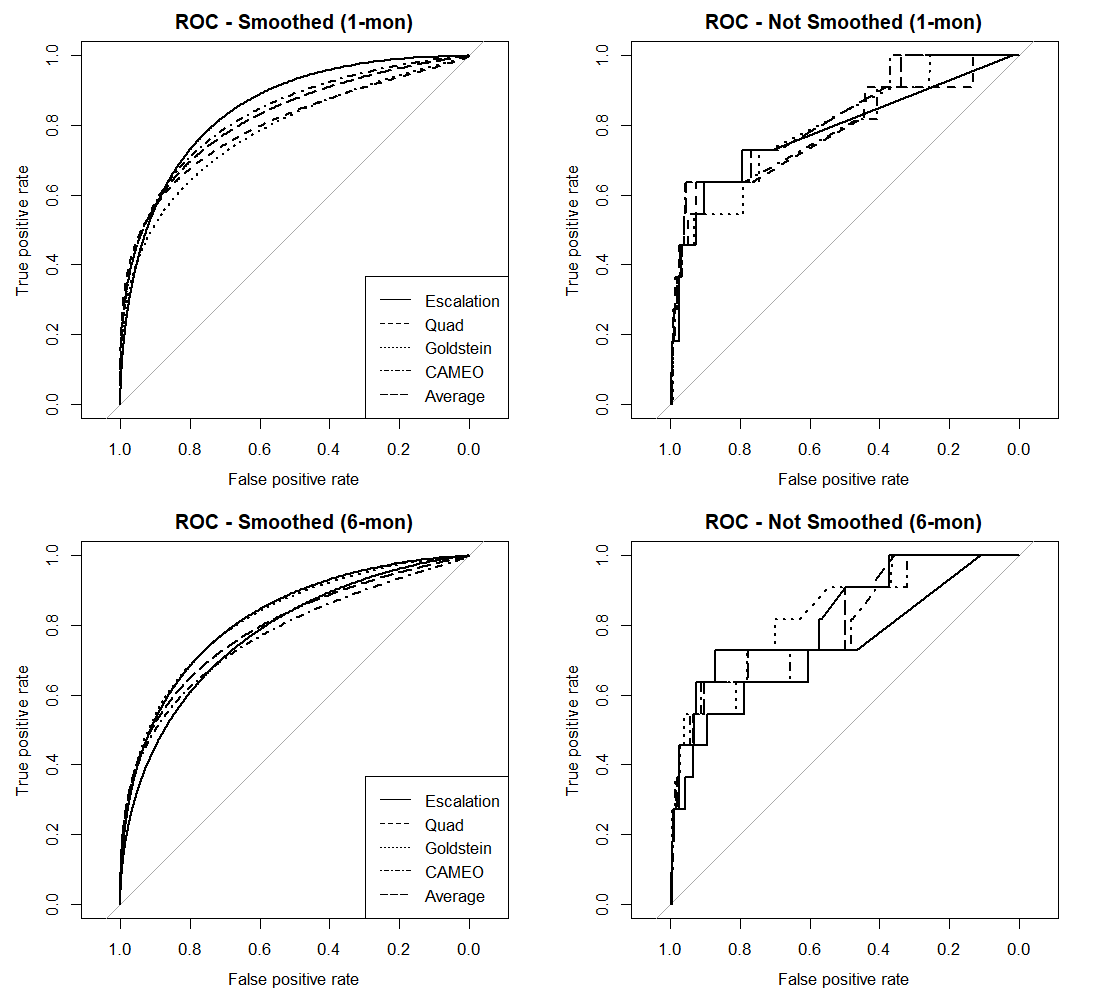
\includegraphics{figures/figure1-replicated.png}
\caption{Replication of BS Figure 1 with both smooth and non-smoothed
ROC curves.}
\end{figure}

ROC curves typically appear step-like in response to the distribution of
positive and negative cases in the data. In this case there are also
groups of cases with identical predicted probabilities, which accounts
for the unusual diagonal lines. In any case, with a sparse outcome like
civil war onsets, the true positive rate on the \emph{y}-axis only
changes when the prediction for a observed positive case is reached. For
these ROC curves, and for that matter in the basic train/test split used
for 12 of the 18 rows/models in BS Table 1, there are only 11 civil war
onset cases in the test set. Thus the ROC curves here are very
step-like, with only 12 (11 positive cases plus 1 for TPR = 0) distinct
\emph{y} coordinates. We can only speculate, but maybe the very
``step''-like nature of the ROC curves plus the presence of unusual
diagonal lines accounts for the decision to use smoothed ROC curves.

As it turns out, this decision has a dramatic impact on the AUC-ROC
calculations. As we will show in the results further below, the
difference between the smoothed and original ROC AUC values is up to
0.12--a huge difference given that row-wise, the models being compared
typically differ by only 0.05 or less--and differentially impacts the
models that are being compared. In fact, BS's original results and
interpretation are entirely conditional on the use of smoothed AUC-ROC.

To our knowledge, the norm is to calculate AUC-ROC values using
original, not smoothed ROC curves. We are in fact not aware of other
work that uses smoothed ROC curves for AUC calculations. It might be
that there are theoretical reasons justifying the use of smoothed ROC
curves over the original ROC curves; but given that this decision
dramatically impacts the interpretation of the BS results, it minimally
would have warranted an explicit discussion in the paper. This is not
the case, and it is only mentioned in the sentence we quote above.

The next three issues we encountered all concern information in Table 2.

\hypertarget{incorrect-weighted-by-pitf-implementation}{%
\subsection{Incorrect ``Weighted by PITF''
implementation}\label{incorrect-weighted-by-pitf-implementation}}

The ``Weighted by PITF'' model is described as follows in BS, page 19:

\begin{quote}
The {[}Weighted by PITF model{]} uses PITF predicted probabilities to
weight the results of the escalation model, ensuring that high-risk and
low-risk countries that happen to take similar values on ICEWS-based
predictors are nonetheless assigned different predicted probabilities in
most months.
\end{quote}

We infer that the intent is that the Escalation model's predictions for
the test set are weighted by the PITF model predictions for the test
set. The implementation actually weighs the test set predictions using
the PITF model predictions for the training set.\footnote{See
  \texttt{1mo\_run\_escalation\_weighted\_PITF.R} line 4, where the PITF
  predictions are taken from the training data set
  (\texttt{train\$pred\_prob\_plus1}). The next line is a hack extending
  the shorter \texttt{weight} vector with missing values to avoid a R
  warning when it is multiplied with the longer vector of escalation
  model test set predictions. Similarly in the 6 month version of this
  file.} This appears to be a coding error.

\hypertarget{incorrect-pitf-split-population-implementation}{%
\subsection{Incorrect ``PITF Split Population''
implementation}\label{incorrect-pitf-split-population-implementation}}

Similarly, the ``PITF Split Population'' model appears to be incorrectly
implemented. BS describe it as, on page 20:

\begin{quote}
The final approach is a random forest analog to split-population
modeling. first compute the average PITF predicted probability for each
country across all years in our training set. We define those that fall
in the bottom quartile as ``low risk'' and the rest as ``high risk.'' We
then run our escalation model on the high-risk and low-risk subsets
separately, combining the results into a single random forest (column
4).
\end{quote}

The intention clearly was to run two separate random forest models, one
each on the low- and high-risk training data splits. The replication
code does indeed run two separate random forecasts, but they are both
run on the exact same training data, which consists of the full training
data all other models are run on. The models are also identical
otherwise, i.e.~they use the same \emph{x} variables and the same random
forest hyper-parameter settings. The \emph{only} difference in the
models as they are implemented in the BS replication code is due to the
non-deterministic nature of the random forest model itself. If we ran
both with the same RNG seed, they would be identical in every respect,
producing identical predictions.\footnote{Disentangling this coding
  error is not straightforward as it occurs over several R scripts and
  requires (or at least is easier to verify by) running partway through
  the actual replication until the objects holding the training data for
  the models are instantiated and can be examined. We have documented
  details at
  \url{https://github.com/rickmorgan2/Blair-Sambanis-replication/issues/5}.}

The implementation error aside, this split-population analog model is
actually quite odd and does not actually replicate an analogue of the
idea behind split-population modeling. Although the two RFs are trained
on separate data (in our updated, fixed replication), the process of
combining them actually just creates a new, larger RF using both
component model's underlying decision (regression\footnote{See further
  below. Although the RF models are used for a binary decision problem,
  the actual implementation uses regression RFs for continuous outcomes.})
trees. Thus while all RF models throughout (except for one of the
robustness checks) are trained with 100,000 decision trees
(\texttt{ntree}), the new RF model after combination does indeed have
200,000 decision trees. Furthermore, the PITF model predictions do not
impact the way the combined RF model predicts at all, not even through a
binary low-/high-risk split. The split-population PITF RF model is
practically speaking just another Escalation model trained with
N=200,000 instead of N=100,000 trees and an extra odd randomization step
added to the already existing RF randomization facilities (row and
column sampling for each decision tree).

\hypertarget{inconsistent-test-set-n-for-the-models-in-table-2}{%
\subsection{Inconsistent test set N for the models in Table
2}\label{inconsistent-test-set-n-for-the-models-in-table-2}}

Lastly, the AUC-ROC values reported in the original BS Table 2 are
calculated on the basis of slightly different numbers of underlying test
set cases (see Table \ref{table2-N}). ROC calculations for a set of
predictions can only be done on the set of cases for which both
non-missing predictions and non-missing outcomes are available. Those
sets differ across models (columns) for each row in Table 2. Thus a
difference in AUC-ROC values for two models could be due to the fact
that they were calculated on different sets of underlying cases, not
because the models are systemically performing at a different level. In
other words, the results for different models in BS Table 2 are actually
not comparable to the other, and any conclusions drawn from such
comparison are potentially incorrect.

We fix this issue by only using predictions for common joint subset of
cases that all models have non-missing predictions for. The original BS
Table 2 1-month have \emph{N}=11,806--12,495 versus a common joint
subset of 9,811, and for the 6-month row \emph{N}=2,070--2,233 versus
\emph{N}=1,915 for the common joint subset.

\hypertarget{incorrect-scoring-of-the-2016-forecasts}{%
\subsection{Incorrect scoring of the 2016
forecasts}\label{incorrect-scoring-of-the-2016-forecasts}}

BS show a confusiong matrix to score their 2016-H1 forecasts in Table 4.
Although the forecasts are for the probability of civil war onset, in
the replication code they are actually scored using the much more common
incidence of civil war, i.e.~including ongoing civil wars as ``1'''s.

The relevant variables in the data are ``incidence\_civil\_ns'' and
``incidence\_civil\_ns\_plus1'', which appears to be a 1-period lead
version of the DV that is used in the actual prediction models. The
incidence DV contains both 0/1 and missing values. By examining the
pattern of missing values, it seems clear that this was originally an
incidence variable indicating whether a country was at civil war in a
given year or not, and which was converted to an onset version so that
onsets retain the value of 1 but continuing civil war years are coded as
missing. This reflects common practice in how these are coded.

By examining the code used to generated Table 4, we were able to confirm
that the onset forecasts are assessed using incidence, not onset. In the
file \texttt{6mo\_make\_confusion\_matrix.do} on line 52, missing values
in ``incidence\_civil\_ns'' are recoded to 1, thus reverting the onset
coding of this variable back to incidence.

\hypertarget{results-of-the-updated-replication}{%
\section{Results of the updated
replication}\label{results-of-the-updated-replication}}

\hypertarget{basic-interpretation-of-table-1}{%
\subsection{Basic interpretation of Table
1}\label{basic-interpretation-of-table-1}}

Table \ref{table1-smooth} is our replication of BS Table 1 with smoothed
AUC-ROC. The results differ slightly from the original BS Table 1,
typically by no more than 0.01, due to the non-deterministic nature of
the RF models. It is the case that BS set the RNG seed in their
replication code, which should theoretically allow exact reproduction,
but (1) there was a change in more recent versions of R that affected
the RNG seeding process, and (2) we refactored the replication script to
allow one to run the models in parallel. In any case, the interpretation
of results should not be sensitive to random variation, i.e.~it should
not depend on using a specific RNG seed. On the basis of these results,
BS conclude that the Escalation model is generally superior to the
alternatives, and we can replicate that interpretation when using
smoothed ROC curves.

\begin{table}[t]

\caption{\label{tab:table1-smooth}Replication of BS Table 1 with smoothed ROC curves; test set AUC-ROC for various models}
\centering
\begin{tabular}{lrrrrr}
\toprule
Model & Escalation & Quad & Goldstein & CAMEO & Average\\
\midrule
\addlinespace[0.3em]
\multicolumn{6}{l}{\textbf{One-month forecasts}}\\
\hspace{1em}Base specification & 0.85 & 0.80 & 0.79 & 0.83 & 0.82\\
\hspace{1em}Terminal nodes & 0.86 & 0.79 & 0.78 & 0.83 & 0.82\\
\hspace{1em}Sample size & 0.85 & 0.81 & 0.70 & 0.86 & 0.84\\
\hspace{1em}Trees per forest & 0.84 & 0.80 & 0.78 & 0.83 & 0.82\\
\hspace{1em}Training/test sets 1 & 0.86 & 0.78 & 0.75 & 0.81 & 0.80\\
\hspace{1em}Training/test sets 2 & 0.81 & 0.79 & 0.72 & 0.78 & 0.78\\
\hspace{1em}Training/test sets 3 & 0.79 & 0.80 & 0.69 & 0.75 & 0.75\\
\hspace{1em}Coding of DV 1 & 0.86 & 0.81 & 0.80 & 0.84 & 0.83\\
\hspace{1em}Coding of DV 2 & 0.92 & 0.81 & 0.81 & 0.82 & 0.81\\
\addlinespace[0.3em]
\multicolumn{6}{l}{\textbf{Six-month forecasts}}\\
\hspace{1em}Base specification & 0.82 & 0.78 & 0.82 & 0.77 & 0.79\\
\hspace{1em}Terminal nodes & 0.80 & 0.75 & 0.81 & 0.75 & 0.77\\
\hspace{1em}Sample size & 0.83 & 0.78 & 0.78 & 0.78 & 0.79\\
\hspace{1em}Trees per forest & 0.82 & 0.78 & 0.82 & 0.77 & 0.79\\
\hspace{1em}Training/test sets 1 & 0.79 & 0.77 & 0.81 & 0.75 & 0.78\\
\hspace{1em}Training/test sets 2 & 0.72 & 0.73 & 0.77 & 0.74 & 0.75\\
\hspace{1em}Training/test sets 3 & 0.88 & 0.70 & 0.81 & 0.68 & 0.79\\
\hspace{1em}Coding of DV 1 & 0.83 & 0.77 & 0.82 & 0.79 & 0.80\\
\hspace{1em}Coding of DV 2 & 0.83 & 0.77 & 0.82 & 0.79 & 0.79\\
\bottomrule
\end{tabular}
\end{table}

Table \ref{table1-nosmooth} shows a version of BS Table 1 with the
conventional non-smoothed ROC curves. The Average model outperforms the
Escalation model in 17 out of 18 cases, and the CAMEO model outperforms
in 16 of 18 cases, with one tie. The Goldstein model generally
outperforms the Escalation model in the 6-month version. The Quad model
appears to be roughly on par with the Escalation model. Thus the
original BS conclusion that the Escalation model is superior to the
alternative models is completely conditional on the non-standard use of
smoothed ROC curves, and overturns when using traditional AUC-ROC
calculations.

\begin{table}[t]

\caption{\label{tab:table1-nosmooth}Replication of BS Table 1 \textit{without} smoothed ROC curves; test set AUC-ROC for various models}
\centering
\begin{tabular}{lrrrrr}
\toprule
Model & Escalation & Quad & Goldstein & CAMEO & Average\\
\midrule
\addlinespace[0.3em]
\multicolumn{6}{l}{\textbf{One-month forecasts}}\\
\hspace{1em}Base specification & 0.78 & 0.78 & 0.79 & 0.80 & 0.82\\
\hspace{1em}Terminal nodes & 0.79 & 0.78 & 0.78 & 0.81 & 0.82\\
\hspace{1em}Sample size & 0.79 & 0.80 & 0.74 & 0.82 & 0.84\\
\hspace{1em}Trees per forest & 0.78 & 0.78 & 0.79 & 0.81 & 0.82\\
\hspace{1em}Training/test sets 1 & 0.78 & 0.76 & 0.76 & 0.79 & 0.80\\
\hspace{1em}Training/test sets 2 & 0.75 & 0.77 & 0.73 & 0.76 & 0.78\\
\hspace{1em}Training/test sets 3 & 0.70 & 0.79 & 0.69 & 0.73 & 0.74\\
\hspace{1em}Coding of DV 1 & 0.80 & 0.79 & 0.80 & 0.82 & 0.83\\
\hspace{1em}Coding of DV 2 & 0.80 & 0.82 & 0.78 & 0.83 & 0.81\\
\addlinespace[0.3em]
\multicolumn{6}{l}{\textbf{Six-month forecasts}}\\
\hspace{1em}Base specification & 0.77 & 0.78 & 0.83 & 0.79 & 0.81\\
\hspace{1em}Terminal nodes & 0.77 & 0.78 & 0.82 & 0.78 & 0.79\\
\hspace{1em}Sample size & 0.78 & 0.77 & 0.80 & 0.80 & 0.82\\
\hspace{1em}Trees per forest & 0.77 & 0.79 & 0.83 & 0.78 & 0.81\\
\hspace{1em}Training/test sets 1 & 0.75 & 0.79 & 0.82 & 0.78 & 0.80\\
\hspace{1em}Training/test sets 2 & 0.70 & 0.75 & 0.78 & 0.75 & 0.77\\
\hspace{1em}Training/test sets 3 & 0.85 & 0.72 & 0.84 & 0.71 & 0.81\\
\hspace{1em}Coding of DV 1 & 0.77 & 0.80 & 0.83 & 0.79 & 0.82\\
\hspace{1em}Coding of DV 2 & 0.80 & 0.78 & 0.84 & 0.80 & 0.81\\
\bottomrule
\end{tabular}
\end{table}

\hypertarget{do-structural-variables-add-to-the-escalation-model}{%
\subsection{Do structural variables add to the Escalation
model?}\label{do-structural-variables-add-to-the-escalation-model}}

Table \ref{table2-fixed} shows our replication of BS Table 2 with (1)
regular, not smoothed, AUC-ROC, (2) fixed ``Weighted by PITF'' and
``PITF Split-Population'' models, and (3) AUC-ROC values computed on the
common joint subset of tests cases that all models have non-missing
predictions for. Table \ref{table2-full} further below shows AUC-ROC
values for both smoothed and non-smoothed versions, and both the
original, model-varying test cases sets and our common joint subset.

\begin{table}[t]

\caption{\label{tab:table2-fixed}Replication of BS Table 2: Test set AUC-ROC for Escalation model with and without structural PITF contribution}
\centering
\begin{threeparttable}
\begin{tabular}{r>{\raggedleft\arraybackslash}p{2cm}>{\raggedleft\arraybackslash}p{2cm}>{\raggedleft\arraybackslash}p{2cm}>{\raggedleft\arraybackslash}p{2cm}>{}p{2cm}}
\toprule
Escalation Only & With PITF Predictors & Weighted by PITF & PITF Split Population & PITF Only\\
\midrule
\addlinespace[0.3em]
\multicolumn{5}{l}{\textbf{One-month forecasts}}\\
\hspace{1em}0.69 & 0.71 & 0.69 & 0.81 & 0.67\\
\addlinespace[0.3em]
\multicolumn{5}{l}{\textbf{Six-month forecasts}}\\
\hspace{1em}0.79 & 0.87 & 0.80 & 0.69 & 0.71\\
\bottomrule
\end{tabular}
\begin{tablenotes}[para]
\item \textit{Note: } 
\item Differences from the original BS Table 2: (1) AUC-ROC values are computed on the common subset of cases, meaning that N is equal in each row; (2) AUC-ROC values are computed using original, non-smoothed ROC curves.
\end{tablenotes}
\end{threeparttable}
\end{table}

BS interpret the results as follows, on page 20:\footnote{We list the
  ``Overall, \ldots{}'' interpretation out of order, last, for clarity.}

\begin{quote}
Of the approaches we test, the split-population analog is most promising
\end{quote}

This is no the case anymore. It outperforms in the 1-month version and
underperforms the Escalation model in the 6-month version.

\begin{quote}
Adding PITF predictors improves the performance of the escalation model
over six-month windows but diminishes it over one-month windows.
\end{quote}

Adding PITF predictors actually improves performance in both cases; the
``With PITF Predictions'' model strictly dominates the ``Escalation
Only'' model.

\begin{quote}
The weighted model performs very poorly regardless.
\end{quote}

It performs roughly on par with the Escalation Only model.

One finding that remains is that the ``PITF Only'' model is outperformed
by the ``Escalation Only'' model. As the former only uses annual inputs,
but the data at hand are the 1-month or 6-months level, this is not
surprising.

\begin{quote}
Overall, our results suggest that while measures of structural risk may
improve predictive performance, the value they add is marginal and
inconsistent. {[}\ldots{}{]} Incorporating PITF thus significantly
reduces or only slightly improves the performance of the escalation
model, regardless of the approach we take.
\end{quote}

The most straightforward method of incorporating the annual, structural
PITF variables--adding them to the predictors of the Escalation RF
model--strictly outperforms the Escalation Only model. Note that the two
other combination models considered are both non-standard, and that the
``PITF Split Population'' model does not in fact actually incorporate
structural information at all. We thus conclude that adding structural
variables actually clearly improves predictive performance.

\hypertarget{the-effect-of-using-smoothed-roc-curves}{%
\subsection{The effect of using smoothed ROC
curves}\label{the-effect-of-using-smoothed-roc-curves}}

\begin{table}[t]

\caption{\label{tab:table1-benefit}Smoothing advantage for BS Table 1: the gain in AUC-ROC when calculated using smoothed ROC curves}
\centering
\begin{tabular}{lrrrrr}
\toprule
Model & Escalation & Quad & Goldstein & CAMEO & Average\\
\midrule
\addlinespace[0.3em]
\multicolumn{6}{l}{\textbf{One-month forecasts}}\\
\hspace{1em}Base specification & 0.07 & 0.02 & 0.00 & 0.02 & 0.00\\
\hspace{1em}Terminal nodes & 0.06 & 0.01 & -0.01 & 0.02 & 0.00\\
\hspace{1em}Sample size & 0.06 & 0.01 & -0.03 & 0.04 & 0.00\\
\hspace{1em}Trees per forest & 0.06 & 0.02 & -0.01 & 0.02 & 0.00\\
\hspace{1em}Training/test sets 1 & 0.09 & 0.02 & -0.01 & 0.02 & 0.00\\
\hspace{1em}Training/test sets 2 & 0.07 & 0.00 & -0.01 & 0.02 & 0.00\\
\hspace{1em}Training/test sets 3 & 0.09 & 0.01 & -0.01 & 0.02 & 0.01\\
\hspace{1em}Coding of DV 1 & 0.06 & 0.02 & 0.00 & 0.03 & 0.00\\
\hspace{1em}Coding of DV 2 & 0.12 & -0.01 & 0.04 & -0.01 & 0.01\\
\addlinespace[0.3em]
\multicolumn{6}{l}{\textbf{Six-month forecasts}}\\
\hspace{1em}Base specification & 0.05 & -0.01 & -0.01 & -0.02 & -0.02\\
\hspace{1em}Terminal nodes & 0.02 & -0.02 & -0.01 & -0.02 & -0.02\\
\hspace{1em}Sample size & 0.05 & 0.00 & -0.02 & -0.01 & -0.03\\
\hspace{1em}Trees per forest & 0.05 & -0.01 & -0.01 & -0.01 & -0.02\\
\hspace{1em}Training/test sets 1 & 0.04 & -0.01 & -0.01 & -0.02 & -0.02\\
\hspace{1em}Training/test sets 2 & 0.03 & -0.01 & -0.02 & -0.01 & -0.02\\
\hspace{1em}Training/test sets 3 & 0.03 & -0.02 & -0.03 & -0.02 & -0.02\\
\hspace{1em}Coding of DV 1 & 0.05 & -0.03 & -0.01 & -0.01 & -0.02\\
\hspace{1em}Coding of DV 2 & 0.03 & -0.01 & -0.01 & -0.01 & -0.02\\
\bottomrule
\end{tabular}
\end{table}

\begin{table}[t]

\caption{\label{tab:table2-benefit}Smoothing advantage for BS Table 2: the gain in AUC-ROC when calculated using smoothed ROC curves}
\centering
\begin{tabular}{l>{\raggedleft\arraybackslash}p{2cm}>{\raggedleft\arraybackslash}p{2cm}>{\raggedleft\arraybackslash}p{2cm}>{\raggedleft\arraybackslash}p{2cm}>{\raggedleft\arraybackslash}p{2cm}}
\toprule
Model & Escalation Only & With PITF Predictors & Weighted by PITF & PITF Split Population & PITF Only\\
\midrule
\addlinespace[0.3em]
\multicolumn{6}{l}{\textbf{One-month forecasts}}\\
\hspace{1em}Base specification & 0.05 & -0.03 & 0 & -0.02 & 0.02\\
\addlinespace[0.3em]
\multicolumn{6}{l}{\textbf{Six-month forecasts}}\\
\hspace{1em}Base specification & 0.06 & -0.01 & 0 & 0.01 & 0.00\\
\bottomrule
\end{tabular}
\end{table}

What impact did the ROC smoothing have overall on the results reported
in BS Tables 1 and 2? Tables \ref{table1-benefit} and
\ref{table2-benefit} show the increase in AUC-ROC when using smoothed
ROC curves, compared to the standard non-smoothed AUC-ROC. Positive
values indicate that smoothing increased a model's apparent performance.
The Escalation model is the only model that consistently had a benefit
from smoothing. For all 8 other models, smoothing sometimes gave a
benefit, sometimes not.

A more dramatic difference stands out when we consider the overall
average impact of smoothing across all flavors of a model reported in
the columns of the tables. The Average, Goldstein, Quad, PITF Split
Population, and Weighted by PITF models are slightly hurt by smoothing,
but on the order of less than 0.01 in absolute magnitude. The ``With
PITF Predictors'' model is hurt on the order of 0.02, i.e.~it appears
substantially worse with smoothing. The CAMEO and PITF Only models
benefit slightly, on the order of 0.01 or less. The Escalation Only
model on the other hand has an average boost of 0.058 to it's AUC-ROC
from smoothing. Considering the spread of AUC-ROC values if we compare
across rows in BS Tables 1 and 2, that boost is substantial.

The use of smoothed ROC curves to calculate AUC-ROC values only clearly
benefits the Escalation model, it does so consistently, and by a
considerable margin. All 8 alternative models reported in Tables 1 and 2
do not on average gain when using smoothed ROC curves to calculate AUC.

\hypertarget{how-accurate-were-the-2016-forecasts}{%
\subsection{How accurate were the 2016
forecasts?}\label{how-accurate-were-the-2016-forecasts}}

\hypertarget{additional-concerns}{%
\section{Additional concerns}\label{additional-concerns}}

\hypertarget{random-forest-hyperparameters}{%
\subsection{Random forest
hyperparameters}\label{random-forest-hyperparameters}}

What initially sparked our interest in the paper was the unusual choice
of hyperparameter settings for the random forest models estimated.

\begin{longtable}[]{@{}llll@{}}
\toprule
Hyperparameter & Default heuristic & Default values (Escalation) & B\&S
value\tabularnewline
\midrule
\endhead
type & & classification & regression\tabularnewline
ntree & & 500 & 100,000 or 1e6\tabularnewline
mtry & \texttt{floor(sqrt(ncol(x)))} & 3 & 3\tabularnewline
replace & & true & false\tabularnewline
sampsize & \texttt{nrow(x)} if replace, & 11,869 & 100 or
500\tabularnewline
& else \texttt{ceiling(.632*nrow(x))} & &\tabularnewline
nodesize & 1 for classification & 1 & 1\tabularnewline
maxnodes & & null & 5 or 10\tabularnewline
\bottomrule
\end{longtable}

There is a stark contrast in the default RF settings and the way Blair
and Sambanis use the RF models. The default approach is to train a
relatively small number (ntree; 500) of classification trees, but where
each tree is fairly big in that it is trained on data that has the same
number of rows as the training data, albeit sampled with replacement
(replace is true; sampsize is 11,869), and allowed to grow fairly deep
(this is governed by nodesize (1), which is the minimum size a terminal
node must have). In contrast, Blair and Sambanis grow very extensive
forests with a large number of trees (100,000 compared to 500), but each
tree is very small and shallow; only a 100 rows are sampled from the
training data for each tree, and the trees are constrained to at most 5
terminal nodes (maxnodes).

This approach only works due to the other unorthodox choice, which is to
use regression, not classification, trees. Trying to use classification
trees with the other parameter settings in fact does not work at all
because it is almost guaranteed that a sample of 100 from the 11,869
training data rows with 9 positive cases will only include 0 (negative)
outcomes in the sample. As it is, using regression with a 0 or 1 outcome
produces warnings when estimating the models:

\begin{verbatim}
Warning message:
In randomForest.default(y = as.integer(train_df$incidence_civil_ns_plus1 ==  :
  The response has five or fewer unique values.  Are you sure you want to do regression?
\end{verbatim}

The RF approach BS use is essentially similar to the probability forests
proposed in Malley 2012. It is not clear if this is intentional or not,
as the paper is not cited.

We tried to create versions of the RF models that use the regular
framework for classification forests, but were unable to create models
that approach the BS RFs test set performance.

How were these hyper-parameter values determined? Do they work better
for some models than others?

\hypertarget{auc-roc-sensitivity}{%
\subsection{AUC-ROC sensitivity}\label{auc-roc-sensitivity}}

RNG and variation

\hypertarget{pre-registration}{%
\subsection{Pre-registration}\label{pre-registration}}

\begin{itemize}
\tightlist
\item
  The escalation model specification, prior to looking at data!
\item
  The hyper-parameter tuning strategy.
\end{itemize}

\hypertarget{conclusion}{%
\section{Conclusion}\label{conclusion}}

BS has a clear misunderstanding of the role that out-of-sample
prediction can plan in analysis. On the one hand it can be used for
simple forecasting while on the other it can be used to evaluate the
performance of models, specifically to overfitting and bias. They
further misrepresent cross-validation which is not about fishing for
results, as claimed by BS. The current state-of-the-art uses prediction
and cross-validation most frequently to provide supportive evidence that
is independent of the estimation procedure and the in-sample data. It is
incorrect to paint this procedure as atheoretical since many studies
will have some explanation for how the model was constructed. These
procedures may simply be used to provide evidence for a theoretical
argument. Though that argument may be unconvincing and/or atheoretical.

The BS approach that is advocated is to use theory to guide prediction.
But theory is a quite ambiguous and undefined concept. It is not a
procedure. What they actually do is to create a model with four right
hand side variables that is supposed to capture a complicated
repression-dissent dynamic. The dynamic is probably not linear, but
their model is. There is a wide-ranging literature on this dynamic that
they do not rely on to construct their model. As such their baseline
comparison is hardly a standard bearer for strong theory.

Further, they complete misunderstand the use of ICEWS event data in
current research. They claim that most uses to date have focused on the
quad categories, but this ignores a wide swath of literature
(Steinert-Threlkeld ApsR 2017) and Metternich et al (AJPX 2013) that
uses a sepcific action---such as protest---defined in the CAMEO
ontology. In the AJPS article we hand coded, for example, every actor in
Thailand and focused on an analysis of how those have been interacting.

We encountered several issues in the code underlying the BS analysis.

The issues we encountered are not subjective modeling choices.

When we fix these issue and perform an updated analysis, the conclusions
BS draw all essentially overturn. In other words, BS findings are based
on a faulty analysis, and invalid.

Using the same analysis BS intend to use, we in fact find that:

\begin{itemize}
\tightlist
\item
  the theory-driven Escalation model is outperformed both by the
  low-effort 1,160 predictor all CAMEO model and the Average ensemble
  model
\item
  structural variables substantially improve the Escalation model's
  performance when added to the pool of predictors the underlying random
  forest model draws on
\end{itemize}

\textbf{AB: add a table comparing BS original claims and updated
results.}

\clearpage

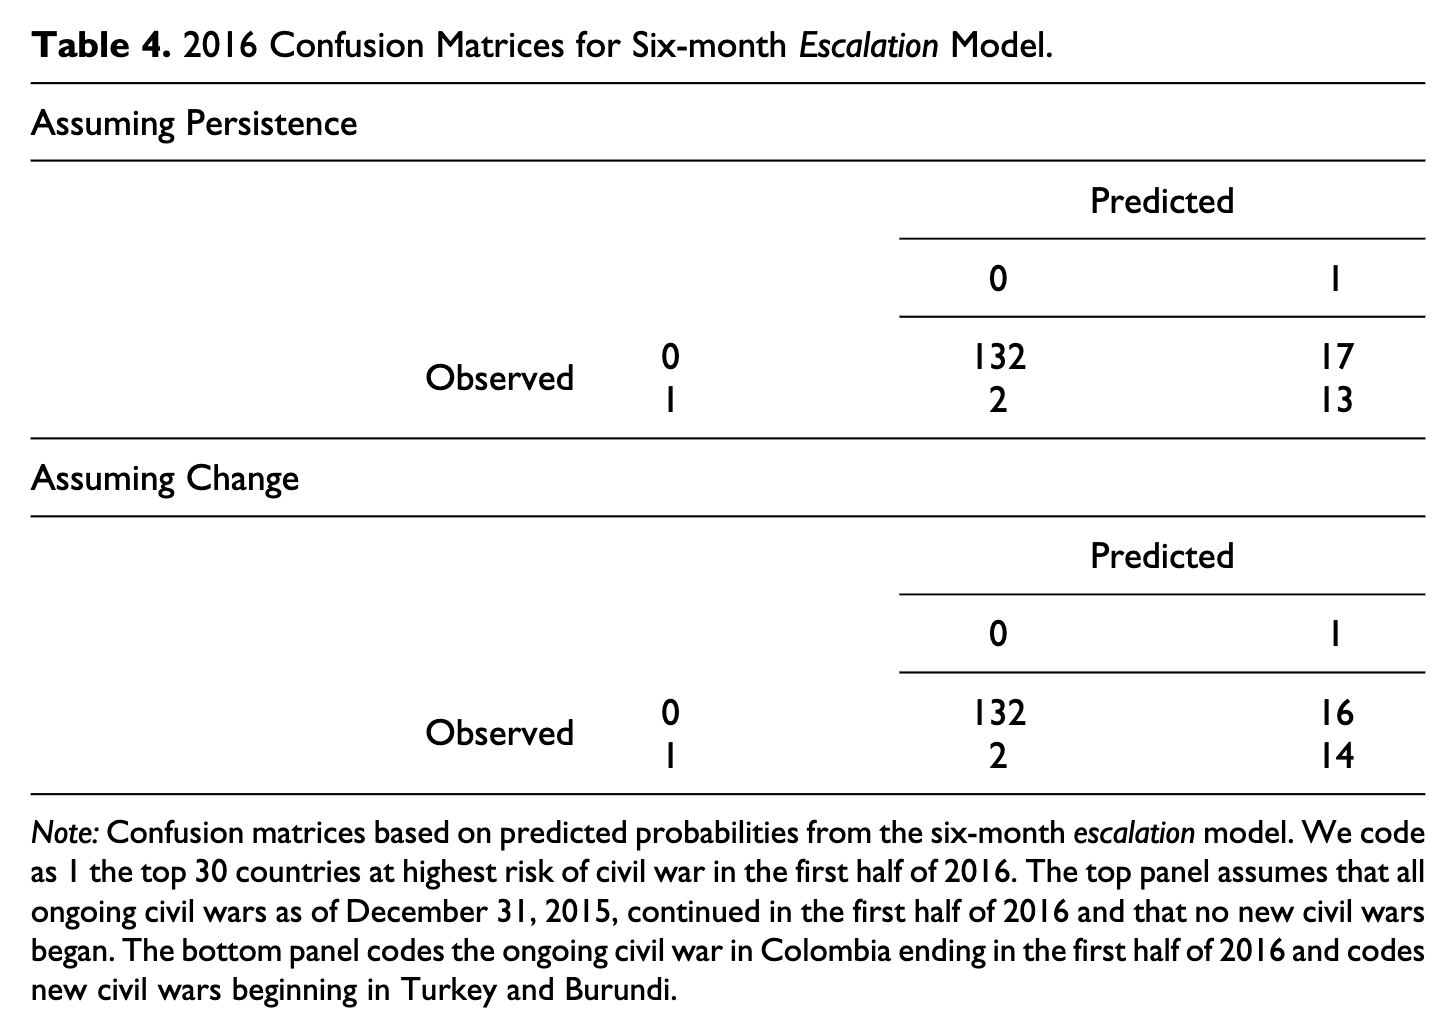
\includegraphics{figures/bands-table4.png}

\begin{table}[t]

\caption{\label{tab:unnamed-chunk-2}2016 Confusion Matrices for Six-month Escalation Model.}
\centering
\begin{tabular}{lrrr}
\toprule
header & Observed & 0 & 1\\
\midrule
 & 0 & 134 & 30\\
\cmidrule{2-4}
\multirow{-2}{*}{\raggedright\arraybackslash Assuming Persistence} & 1 & 0 & 0\\
\cmidrule{1-4}
 & 0 & 134 & 28\\
\cmidrule{2-4}
\multirow{-2}{*}{\raggedright\arraybackslash Assuming Change} & 1 & 0 & 2\\
\bottomrule
\end{tabular}
\end{table}

\begin{table}[t]

\caption{\label{tab:table2-N}Number of valid test predictions for each cell in BS Table 2}
\centering
\begin{tabular}{ll>{\raggedleft\arraybackslash}p{2cm}>{\raggedleft\arraybackslash}p{2cm}>{\raggedleft\arraybackslash}p{2cm}>{\raggedleft\arraybackslash}p{2cm}>{\raggedleft\arraybackslash}p{2cm}}
\toprule
 & Horizon & Escalation Only & With PITF Predictors & Weighted by PITF & PITF Split Population & PITF Only\\
\midrule
\addlinespace[0.3em]
\multicolumn{7}{l}{\textbf{Original model-specific cases}}\\
\hspace{1em} & 1 month & 13748 & 13155 & 13461 & 13748 & 13510\\
\cmidrule{2-7}
\hspace{1em} & 6 months & 2366 & 2264 & 2317 & 2366 & 2265\\
\cmidrule{1-7}
\addlinespace[0.3em]
\multicolumn{7}{l}{\textbf{Cases adjusted to common subset}}\\
\hspace{1em} & 1 month & 9811 & 9811 & 9811 & 9811 & 9811\\
\cmidrule{2-7}
\hspace{1em} & 6 months & 1915 & 1915 & 1915 & 1915 & 1915\\
\bottomrule
\end{tabular}
\end{table}

\begin{table}[t]

\caption{\label{tab:table2-full}Replication of BS Table 2 with smoothed/original ROC and with original varying N cases or adjusting for common case set with constant N}
\centering
\begin{tabular}{ll>{\raggedright\arraybackslash}p{1.5cm}>{\raggedleft\arraybackslash}p{2cm}>{\raggedleft\arraybackslash}p{2cm}>{\raggedleft\arraybackslash}p{2cm}>{\raggedleft\arraybackslash}p{2cm}>{\raggedleft\arraybackslash}p{2cm}}
\toprule
 &  & Smoothed ROC & Escalation Only & With PITF Predictors & Weighted by PITF & PITF Split Population & PITF Only\\
\midrule
\addlinespace[0.3em]
\multicolumn{8}{l}{\textbf{Original model-specific cases}}\\
\addlinespace[0.3em]
\multicolumn{8}{l}{\textit{1 month}}\\
\hspace{1em}\hspace{1em} &  & Yes & 0.85 & 0.76 & 0.80 & 0.81 & 0.77\\
\cmidrule{3-8}
\hspace{1em}\hspace{1em} &  & No & 0.78 & 0.77 & 0.80 & 0.80 & 0.75\\
\cmidrule{2-8}
\addlinespace[0.3em]
\multicolumn{8}{l}{\textit{6 months}}\\
\hspace{1em}\hspace{1em} &  & Yes & 0.82 & 0.86 & 0.81 & 0.79 & 0.74\\
\cmidrule{3-8}
\hspace{1em}\hspace{1em} &  & No & 0.77 & 0.86 & 0.81 & 0.82 & 0.74\\
\cmidrule{1-8}
\addlinespace[0.3em]
\multicolumn{8}{l}{\textbf{Cases adjusted to common subset}}\\
\addlinespace[0.3em]
\multicolumn{8}{l}{\textit{1 month}}\\
\hspace{1em}\hspace{1em} &  & Yes & 0.74 & 0.68 & 0.69 & 0.80 & 0.69\\
\cmidrule{3-8}
\hspace{1em}\hspace{1em} &  & No & 0.69 & 0.71 & 0.69 & 0.81 & 0.67\\
\cmidrule{2-8}
\addlinespace[0.3em]
\multicolumn{8}{l}{\textit{6 months}}\\
\hspace{1em}\hspace{1em} &  & Yes & 0.85 & 0.86 & 0.79 & 0.70 & 0.71\\
\cmidrule{3-8}
\hspace{1em}\hspace{1em} &  & No & 0.79 & 0.87 & 0.80 & 0.69 & 0.71\\
\bottomrule
\end{tabular}
\end{table}

\hypertarget{references}{%
\section*{References}\label{references}}
\addcontentsline{toc}{section}{References}

\hypertarget{refs}{}
\leavevmode\hypertarget{ref-blair2020forecasting}{}%
Blair, Robert A., and Nicholas Sambanis. 2020. ``Forecasting Civil Wars:
Theory and Structure in an Age of `Big Data' and Machine Learning.''
\emph{Journal of Conflict Resolution}.


\end{document}
